\documentclass[journal]{IEEEtran}

\renewcommand\thesection{\arabic{section}} 
\renewcommand\thesubsectiondis{\thesection.\arabic{subsection}}
\renewcommand\thesubsubsectiondis{\thesubsectiondis.\alph{subsubsection}}
\renewcommand\theparagraphdis{\arabic{paragraph}.}

%\usepackage[retainorgcmds]{IEEEtrantools}
%\usepackage{bibentry}  
\usepackage{xcolor,soul,framed} %,caption

\colorlet{shadecolor}{yellow}
% \usepackage{color,soul}
\usepackage[pdftex]{graphicx}
\graphicspath{{../pdf/}{../jpeg/}}
\DeclareGraphicsExtensions{.pdf,.jpeg,.png}

\usepackage[cmex10]{amsmath}
%Mathabx do not work on ScribTex => Removed
%\usepackage{mathabx}
\usepackage{array}
\usepackage{mdwmath}
\usepackage{mdwtab}
\usepackage{eqparbox}
\usepackage{url}
\hyphenation{op-tical net-works semi-conduc-tor}
\usepackage{graphicx}



%\bstctlcite{IEEE:BSTcontrol}
%=== TITLE & AUTHORS ====================================================================
\begin{document}

\bstctlcite{IEEEexample:BSTcontrol}
    \title{
\includegraphics[width=2.5in]{photo/0_cityu} \\
     How can the effectiveness of marketing \\ be improved ‘Airbnb Seattle’? \\ 
     \textit{Dataset of 2016}
     }

  \author{LIST Nicole ,
      L\"OHR Tim,
      BOHNSTEDT Timo,\\
      PANG Tsz Ching 
      and BAL Kiran Jeniffer% \\ <-this % stops a space
}

% The paper headers
\markboth{Project Report
Machine Learning for Business IS4861 
}{Roberg \MakeLowercase{\textit{et al.}}}


% ====================================================================
\maketitle
% === ABSTRACT 
\begin{abstract}
%\boldmath
This paper should present, how the marketing effectiveness of Airbnb can be enhanced by the analysis of a dataset of 2016. In order to improve the marketing, the four Ps of the marketing-mix should be addressed. The dataset contains listings of rented apartments and their attributes. The data for the first P, Product, is analyzed by using a WordCloud (obtained by using a Natural Language Processing) the 50 most mentioned words of all reviews on the apartments are displayed according to their neighborhood. Findings for the Price Policy are obtained by using Linear Regression a Neural Network and an Extra Tree classifier, which extracts the features that influence the price have been used. In order to find out when a marketing campaign should be started, the number of visitors over the year is analyzed and a prediction for 2017 is made by Linear Regression. Our findings show, that lessors should put words like “park”, “walk”, “lake” or “downtown” into their description to successfully address their target group. The price for an apartment is dependent of the attributes listed in the dataset, with number as review as attribute with the highest correlation. A good point in time to start a campaign would be February, as the number of visitors starts to decrease in March.
\end{abstract}

% === KEYWORDS 
\begin{IEEEkeywords}
\hl{kaggle, machine learning, business, data analytics, airbnb}
\end{IEEEkeywords}

\IEEEpeerreviewmaketitle

% === I. Project background and motivation
\section{Project background and motivation}
\noindent \begin{itshape}"Brian, I thought of a way to make a few bucks - turning our place into "designers bed and breakfast" - offering young designers who come to town a place to cra during the 4 day event, complete with wireless Internet, a small desk space, sleeping mat, and breakfast each morning. Ha Joe! \\
\end{itshape}
\IEEEPARstart{T}{}his simple email, sent on September 22 in year 2007, has been the start of an equally simple business, which has been started in 2008 and is 31 billion dollar worth today. In 2007 two locals from San Francisco decided to host visitors of the design conference, which took place in their hometown. This simple concept has been the impulse to create a platform, where private people can offer and rent out their accommodation to visitors. According to the basic idea, the platform is called Airbnb, the short form for 'Airbed and Breakfast' and a new company, which should become very successful was born. Since the company founding, the Airbnb community became more than just an opportunity to earn some extra money by renting out an accommodation, or to find a cheap place to stay. According to the company’s website, today it is about 'sharing' and having the possibility to 'experience' a town. In 2016, Airbnb stresses this in their marketing campaign 'Don't go there. Live there!'. Over the time the platform provided the possibility to offer tours and activities. So, locals can show their culture and city in another and special way to visitors than only renting apartments. As 11 years have passed since the company has been founded, Airbnb announced to start a new chapter by becoming a public-tradable company in 2020. So, in the future the stockholders will show great interest in the revenue and prognoses of the company and therefore, the company needs to present good predictions for the next years. Furthermore, it should reveal a plan how to increase its business value and reach its aims, set at the beginning of the year. At this point data collection and analysis is very important. Analyzing customers' and company’s past behavior can be used to predict the further development of the company and help to find the right instruments to reach the companies' aims. One major goal of companies is to increase their revenue or at least to increase their customer base. To have a good marketing is essential for Airbnb to reach the yearly goal as the quality of marketing is one of the factors, which influences the increase of number of customers.\\
By definition marketing is about the firm’s effort to address customer needs and expectations, which influences the demands made by the customers on the product and need to be fulfilled by the product \cite{schiernbeck}. So, it is also about the tradeoff of ‘evoking’ needs and expectation of consumers on a level that the product can satisfy and is able to compete with competitive product. In order to find the essential requirements, applying marketing instruments like the marketing mix can be helpful. The marketing mix consists of four policies: Product, Price, Promotion and Place. Having a good data foundation and analysis is important, as we can deduce future customer needs and behavior by analyzing the requirements of past visitors and therefore we can base our marketing assumptions within the four policies on solid data.\\
In our paper we analyze a dataset containing information on rented accommodations in Seattle in the year 2016. As already mentioned the company will aim for good predictions in 2020, in order to present them to shareholders, the company will aim to obtain high quality data to base a marketing campaign on. As the dataset is of 2016, we actually can not make proper predictions for the year 2020 and therefore will not be able to deliver the information on the future development of the company in 2020. Nevertheless, analyzing this dataset is useful in order to improve the marketing of Airbnb and therefore can contribute to a positive company development also in year 2020, if the right instruments can be chosen according to our analysis. The following sections will 
\begin{enumerate}
\item raise some questions, which need to be answered, in order to give suggestions on the design of a marketing campaign
\item the dataset will be presented and visualized. The used models will be described and analyzed
\item findings and their impacts on a suggested marketing strategy will be presented and the questions raised up will be answered\\
\end{enumerate} 

\noindent Before we start to describe how we analyzed our data according to each single policy, we explain the general idea of each policy and apply the general idea on Airbnb
\subsection{Product}
\noindent As already mentioned before, marketing is about fulfilling customer needs and expectations. Within product policy the aim is to understand one’s market and be able to figure out which needs and wants the customers have. In general, one can say that the main need of travelers is to find an accommodation but nowadays it is not only about finding accommodations but even more about discovering the right accommodation. It is not only having a nice and clean room bathroom, with white and clean towels and bead sheets. The surrounding and flair of the accommodation becomes more and more important. This issue Airbnb has already addressed in its advertising spot \cite{RN6}, so Airbnb is aware of the wants of travelers and is responsive to this in its advertisement. Thinking a step further, it is not enough to just show the customer that renting Airbnb apartments is a nice way to ‘really live’ there instead of just ‘go there’. When the customer has been attracted by Airbnb to search for on apartment on their website it is important to present the apartment in a good way. Therefore, the description of the apartments should mention all aspects the customer considers as important.
\subsection{Price}
\noindent The price of a product is a very important aspect regarding the marketing of a product. If customers consume a product on a certain price level, their willingness to pay is higher than the price level. This means that they expect the value they obtain by purchasing is higher than their cost and therefore they accept paying a certain price. So for a certain price level the customer expects to obtain a certain value and therefore immediately raises some expectation the product needs to fulfill in order to satisfy the customer. So if a visitor decides to rent an apartment at a certain price level, this customer will have certain expectations. If these are not fulfilled by the apartment the customer will have a negative experience and might not book his next holiday accommodation on Airbnb. In order to prevent this scenario, Airbnb could support the lessors in determining the perfect price level for their accommodation, by letting them know, which attributes have a high value for visitors.
\subsection{Promotion}
\noindent For Promotion Policy it is important to find out when advertisement should issue a marketing campaign and which content to bring up. The aim of this is obvious: we need to be able to make suggestions, which advertise content will address future visitors and when it will be the best to effectively reach the customer. So far our suggestions mainly focused on suggestions for (former) lessors how they can improve renting their apartment. In this section we want to give Airbnb some suggestions, what a successful marketing campaign could look like. Of cores also single lessors could promote their apartment on other channels as well, so the tips we provide for Airbnb can probably also be applied by lessors it self but for now we want to focus on the suggestions for Airbnb.
\subsection{Place}
\noindent The Place Policy considers where customers get in touch with the product and consume it, in order to find a suitable retail location that is accessible for customers. The first contact between lessor and renter happens on Airbnb but the final ‘purchase’ of the product, takes places in Seattle. As Airbnb is a platform, which acts as agent between lessor in Seattle and renter, we do not need to care about this in our data analysis, as this fact is fixed and can not be changed.

% === II. Procedural Method==================================== 
\section{Procedural Method}
\noindent In this section the four areas of the marketing-mix will be described and how our data analysis can contribute to improve the marketing of Airbnb in Seattle according to each policy of the marketing-mix.\\\\\noindent The dataset we are going to analyze contains several information about the renting of apartments via the platform Airbnb in Seattle. \\\\ As Airbnb is an agent for lessors, who want to rent their apartment to tourists, it earns its money by receiving a commission for every rented apartment. Therefore, Airbnb should aim for a high booking rate to increase their own profit. That is one reason, why Airbnb should care which apartments are offered on their platform and how they are presented (e.g. by the description, price, …). So, it can make sense for Airbnb to give lessors some suggestions how to promote and present their accommodation to achieve a maximal booking rate. Deducted of this assumption, we want to provide some suggestions for lessors to promote their apartments in the perfect manner but also want to give some suggestions, what point in time is best for Airbnb to release a marketing campaign to advertise some apartments in Seattle. 

\subsection{Product}
\noindent By our data analysis we would like to support the lessors in creating a good and appealing description. By analyzing the reviews of customers and filtering the 50 most mentioned words, we can conclude that these mentioned words are important to customers and therefore lessors should mention them in their description. As Seattle is a huge city with lots of different areas with different style and flairs, we conduct word clouds for every neighborhood, which represent how often a word of the 50 chosen ones occurs. This offers the advantage that we can better address and select certain customer groups. A neighborhood, with lots of parks, is probably better for nature lover than for reveler. So, nature lovers will mention the parks in their reviews very often and according to our word cloud (which is based on the reviews), lessors in this neighborhood will focus on the parks nearby their accommodation. If a person, who prefers partying at night, reads this description his or her interest will not be raised and therefore the person will search for apartments in another neighborhood. This creates an ‘automatic’ selection and increase the chance that a customer finds an apartment in a neighborhood, which fits his/ her interest. So, a first question we would like to answer is: \begin{itshape}Which facts lessors need to address in their description to raise the interest of potential customer, who ‘fit’ the vibe of the neighborhood and set their focus on the same aspects as former customers of these apartments?\end{itshape}

\subsection{Price}
\noindent As already mentioned Airbnb should support lessors to find the right price level for an appartment. By analyzing our dataset, it will be possible to determine the correlation between attributes and price. The attributes with the highest correlation are the most important to an average customer. By knowing the most important attributes a lessor can compare these attributes of his own accommodation with other accommodations and consider on which price level other apartments have been rented out or are offered. So it becomes easier for lessors to get an overview by focusing on the appropriate set of attributes. Based on the first question we need to answer:
\begin{itshape}
Which attributes have the highest impact on the charged price of an apartment?
\end{itshape}\\
Furthermore, we would like to indicate the price trend of the rented apartments. Lessors can see during which season prices increase or decrease and can adapt their prices to the overall price variability. This makes the lessors yield an optimal return and increase their booking rate, as the price is neither too expensive nor too cheap. So, our next question to answer will be:
\begin{itshape}
When can lessors increase the price per night for their apartment and when should they lower it?
\end{itshape}\\
Helping the lessors to set the perfect price level might even help to secure the existence of Airbnb, as lessors do not quit to offer their accommodation on Airbnb as they have too low revenues (because of too low renting prices of too less customers - due to high prices).
To estimate the price we used a neural network, but we scored fairly bad compared to another paper. This leads to the question:
\begin{itshape}
Why did our neural network score so much worse than the neural network of the paper Predictive modelling on Airbnb listing prices \cite{RN1}?
\end{itshape}
%=====================================================
\subsection{Promotion}
\noindent For this section, some information deduced for the previous two sections will be reused. As already mentioned, the word clouds represent the features customers value the most and therefore a marketing campaign should address these issues.\\
The Promotion Policy does not only focus on the content of the marketing campaign but also when the campaign will be most effective. In order to give an indication regarding that issue, we would like to analyze the booking rate and predict it for the next year. So it becomes visible, when there will be phases with a lower booking rates. Shortly before that phase the campaign should be started in order to motivate people to book their apartment on Airbnb and keep the booking level up. So, regarding the Promotion Policy the two question of interest are:
\begin{itshape}
Which content should a marketing campaign have?
What is a good point in time to start a marketing campaign?
\end{itshape}
According to the Promotion Policy a second issue is to decide where/ via which tools the marketing campaign should be distributed and be presented to potential customers. As our dataset does not give any information on the fact how customers got to know of Airbnb or for which reason they decided to book their accommodation on Airbnb, we decided to neglect the aspect of Promotion Policy, as we can not yield any results or deduce some information, which would be helpful to decide on the distribution channel of our marketing campaign. 
%
%==================================================
%
\section{Executive summary} 
\noindent The aim of this report is to find out how the effectiveness of marketing ‘Airbnb Seattle’ can be improved. This report orients itself at the four Ps from Marketing Mix, which are Product, Price, Place and Promotion. 
The data originally consisted of three data sheets Listing, Reviews and Calendar and had to be prepared for the analyzation. 
The analysis wants to answer the following six questions: 
%==================================================
\begin{itemize}
\item Why did our neural network score so much worse than the neural network of the paper \textit{Predictive modelling on Airbnb listing prices} \cite{RN1} ?
\item Which facts lessors need to address in their description to raise the interest of potential customer, who ‘fit’ the vibe of the neighborhood and set their focus on the same aspects as former customers of these apartments?
\item Which attributes have the highest impact on the charged price of an apartment?
\item When can lessors increase the price per night for their apartment and when should they lower it?
\item Which content should a marketing campaign have?
\item What is a good point in time to start a marketing campaign?
\end{itemize}
%==================================================
The analysis yields out  which keywords lessor should use best to put into their accomondation description such such as parks, shops, restaurant, etc.
Furthermore, the amount of positive reviews are vital for possible renters being interested in ones listing. How long the lessors are active is also an important factor. 
Host\_response\_time, host\_response\_rate and host\_acceptance\_rate are the most important indicators if and at which price the accomondation gets booked. The number of bathrooms, bedrooms and beds together have an influence on pricing as well. 
%
% === II. 4	Data description with visualization==========================
%
\section{Data description with visualization}
\subsection {General}
\noindent Our dataset consists of three excel sheet: ‘listings.csv’, ‘calendar.csv’ and ‘reviews.csv’.\\
Listings consists of 92 attributes with 3,818 data entries. Every single row represents one apartment in Seattle that has been offered for rent via the platform of Airbnb. Calendar consists of 1,393,570 data entries and 4 columns. The dataset connects a certain time period with an apartment and indicates whether it has been rented out or been available during that period. The last dataset ‘reviews.csv’ contains all reviews former visitors have handed in for an apartment, it contains the reviewer’s Id, name comments, the date as well as the house ID.\\So, if the excel sheets are combined it can be deducted the following information: the key facts about an apartment (like the size, prize, number of beds, usable facilities, …), furthermore one can get a general idea about, what the apartment looks like by the description (written by the lessor) as well as by the reviews (written by former guests) and it is known when the apartment has been available or rented.
%
%==================================================
%
\subsection {Data preprocessing}
\noindent First of all, we computed how many different values certain attributes can have. Therefore, we computed a table that listed the attribute name as well as how many unique attribute values exist for that attribute. In a following step we replace all na-values by suitable possible values. In order to be able to use the data in the following steps and analyze it in a proper way. To be able to fit our models, we replaced some textual values by numerical ones and split the dataset into a training dataset and a test dataset. The training dataset we will use to ‘create’ or models in order to check our created models and be able to see how good for example predictions will be and which error we need to expect we need the test data.
%
%==================================================
%
\subsection {More detailed dataset description}
\noindent \subsubsection{Listings}  The listing dataset consists of 92 columns, with attributes that describe different characteristics of the rented apartments. It describes 3818 apartments that are allocated in 79 neighborhoods. Combined with the review dataset it represents a dataset, which can be used to find some attributes, valued as most important by customers. If it is combined with the calendar dataset, a data analysis can help to determine the factors which are important to, not only attract visitors, but also to finally rent it out successfully. Especially we will use this combination to find out which attributes of the apartments did influence the price charged the most. The Figure \ref{districts_room_types} shows the districts with the most offers, spitted by their room type.
%
%Figure
\begin{figure}
  \begin{center}
  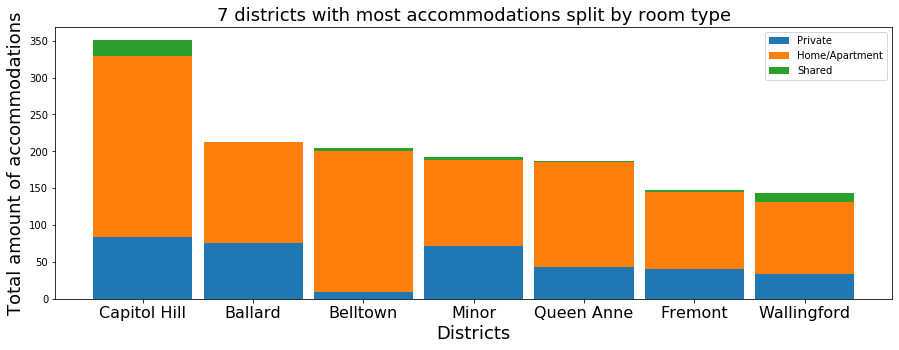
\includegraphics[width=3.5in]{photo/4_most_acc_split_by_roomtype.png}\\
  \caption{Seven districts with most accommodations split by room type}\label{districts_room_types}
  \end{center}
\end{figure}
\subsubsection{Reviews}
%
In order to have an insight whether the reviews are written by satisfied or rather unsatisfied visitors, we computed a bar chart which shows the rating-number of reviews ratio. (Figure \ref{score_reviews_ratio})
%
%Figure
\begin{figure}
  \begin{center}
  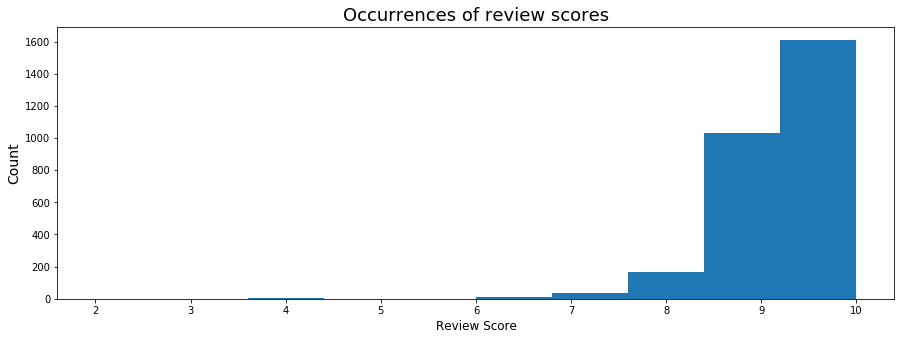
\includegraphics[width=3.5in]{photo/2_1_occurences_of_review_scores.png}\\
  \caption{Score and number of reviews ratio}\label{score_reviews_ratio}
  \end{center}
\end{figure}
%

%
%Figure
\begin{figure}
  \begin{center}
  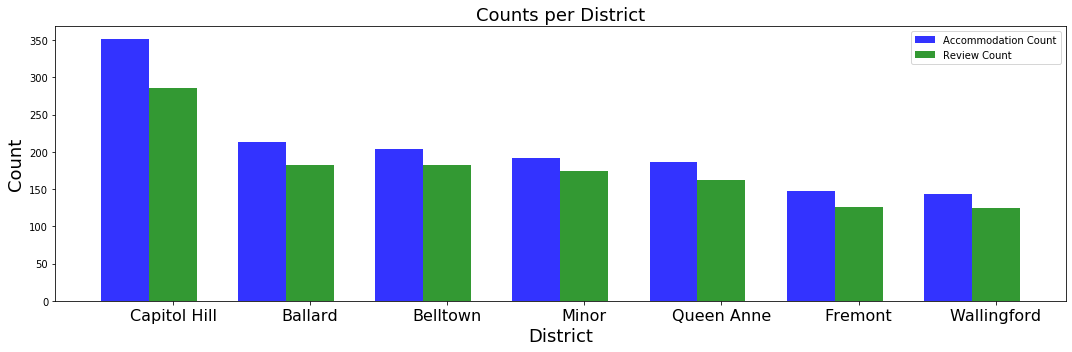
\includegraphics[width=3.5in]{photo/3_count_per_district.png}\\
  \caption{Compare review and accommodation count}\label{review_district}
  \end{center}
\end{figure}
%

Besides, it shows that most of the reviews give the highest value possible (10) and there are hardly no reviews that give a rating value lower than (8). So, in our further analysis we assume that the reviews are written in a rather positive tone and we need to keep in mind that the reviews have been written by overall satisfied tourists. Besides, it shows that most of the reviews give the highest value possible (10) and there are hardly no reviews that give a rating value lower than (8).\\ 
Another comparison shows the amount of reviews depending on the neighbourhood \ref{review_district}. We can see a direct correlation between those two feature. Apparently there is no district which gets less reviews because of any special reason. \\

First we had the idea of creating a new feature called \textit{Sentiment} for each review. It should be calculated with a Sentiment Analysis and label each review with a score. By reading the related work of the Seattle-Dataset, we noticed that another group already researched this idea. They used the Microsoft Azure Sentiment Analysis API to label each review with a score between 0 to 100. Unfortunately the team found out, that this feature has no relevant impact on predicting the price \cite{RN1}, because as shown in figure \ref{score_reviews_ratio}, nobody found a Gaussian-Distribution or any other useful distribution for the reviews so far.\\
In order to make sure that there is no correlation between the number of reviews and the review score of apartments in a certain neighborhood, we generated a figure which shows that relationship (Figure \ref{compare_the_neighbourhoods}). \\
%
%Figure
\begin{figure}
  \begin{center}
  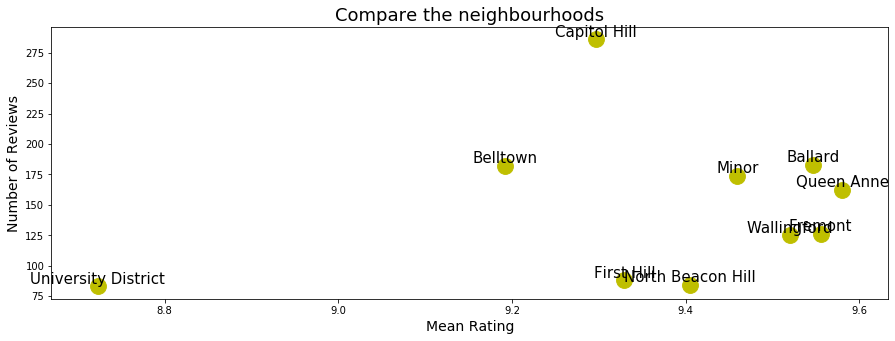
\includegraphics[width=3.5in]{photo/2_2_compare_the_neighbourhoods.png}\\
  \caption{Mean rating and number of reviews ratio (per neighborhood)}\label{compare_the_neighbourhoods}
  \end{center}
\end{figure}
%

%Figure
\begin{figure}
  \begin{center}
  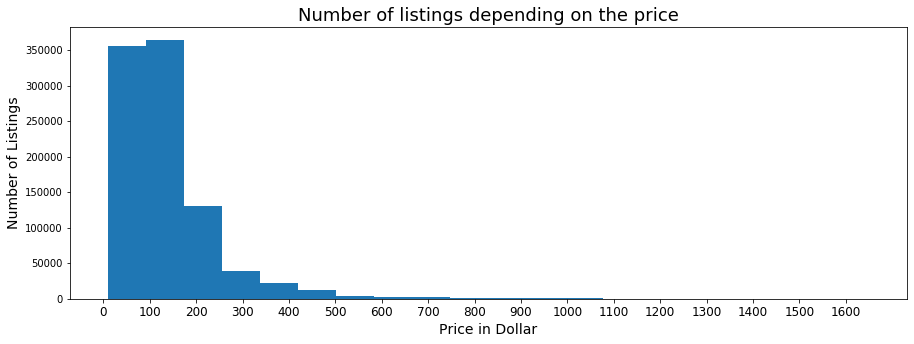
\includegraphics[width=3.5in]{photo/1_number_of_listings_depending_on_price.png}\\
  \caption{Mean accommodation price with count}\label{mean_acc}
  \end{center}
\end{figure}
%

In this figure it becomes visible that neighborhoods, whose apartments in total got 50 to 100 reviews score a mean rating of about 9.2 to 9.7. Approximately the same mean rating is also achieved by district where the apartments are rated 125 to 300 times. There is only one outlier (‘University District’), which scored al pretty low mean rating value compared to all other districts. As this is the only outlier, we will neglect this in our following assumptions.
To sum up, we can conclude that both figures (\ref{score_reviews_ratio} and \ref{compare_the_neighbourhoods}) show that the mean rating for every district is relatively high and a high value is not dependent on the number of reviews for a certain district. For a better comparison we provide figure \ref{mean_acc} to show all the provided accommodation with their according prices.
\subsubsection{Calendar}
\noindent This part of the data shows, when certain apartments are available and when they are rented out. Within our analysis we assume, that an apartment, which is listed as ‘not available’ in the ‘calender.csv’ is occupied by a visitor. If it is ‘available’ we assume that the owners would have liked to rent the apartment out but there has not been any visitor renting it. In figure \ref{occupied_ratio_appartments} the ratio of occupied and available apartments in 2016 is presented.
%
%Figure
\begin{figure}
  \begin{center}
  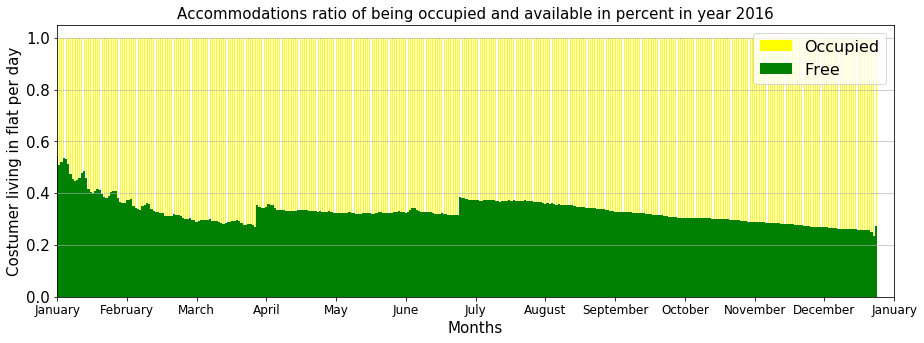
\includegraphics[width=3.5in]{photo/11_acc_ratio_occupied.png}\\
  \caption{occupied ratio of appartments}\label{occupied_ratio_appartments}
  \end{center}
\end{figure}
%
While in January only half of the apartments have been occupied, the number of rented apartments raised until April when a sudden drop in rented apartments appeared. The same procedure repeats in July. After that second drop the number of occupied accommodations raises again. Nevertheless, it has to be mentioned that the percentage of free apartments never exceeds 40\% after February anymore but also never drops below 20\%. At this point the question, whether there is a correlation between the degree of booking and a ‘perfect’ description exists and therefore the percentage of free apartments can be decreased by mentioning the right aspects in the description. 

\section{Models}
\subsection{Natural Language Processing}
\noindent NLP stands for natural language processing. We can use this technique to process and analyze natural language data from the reviews of our dataset. NLP breaks down language into tinier, elemental pieces, trying to understand the relationships between the pieces and explore how the pieces are related together to generate meanings and conclusions out of it. To perform analysis, we encounter plenty of steps called the preprocessing. Most of this steps can be solved with multiple python packages. We decided to use the NLTK package, because it provides an easy to use dashboard and contains all of the required preprocessing methods.
The preprocessing steps for transforming the reviews into Wordclouds are below with exactly this sequence of steps:
\begin{itemize}
 \item Regular Expression Tokenizer
 \item Stopwords for English + two additional Words “Seattle” and “Neighbourhood”
 \item Lowercase
 \item WordNetLemmatizer
\end{itemize}

\subsubsection{Regular Expression Tokenizer}
\noindent This  tokenizer uses a regular expression term with the intention of cleaning the text completely from any punctuation marks and unnecessary spaces.  The expression r'\textbackslash +' does exactly this, because it avoids every character which is not alphanumeric (A-Z, numbers) and underscore (\_) or an asterisk (*). Everything else will get omitted by the regular expression. The Tokenizer itself detects the ASCII character for the space and splits in this way the words from each other to store it in an array.

\subsubsection{Stop Words}
\noindent A Text normally contains stop words like ‘the’, ‘is’, ‘are’. Stop words should be filtered from the text to be processed in the best way. There is not an universal list of stop words in NLP research, however the nltk module contains a list of stop words.

\subsubsection{Lowercase}
\noindent This is just the built-in pyton method .lower() which can be used to turn strings into lowercase.

\subsubsection{WordNetLemmatizer}
\noindent Lemmatization is the process of turning the words into their base form. There is a second almost similar approach called stemming. 
The difference between stemming and lemmatization is, lemmatization looks at the context oft he word and transforms it to its base form, whereas stemming just removes the last few characters. Unfortunately this often leads to incorrect spelling and meaning errors. For example, lemmatization would properly identify the base form of ‘caring‘ to ‘care’, whereas, stemming would cutoff the ‘ing’ part and convert it to car.
\begin{itemize}
\item Caring with \textit{Lemmatization} into Care
\item Caring with \textit{Stemming} into Car
\end{itemize}

%Figure
\begin{figure}
  \begin{center}
  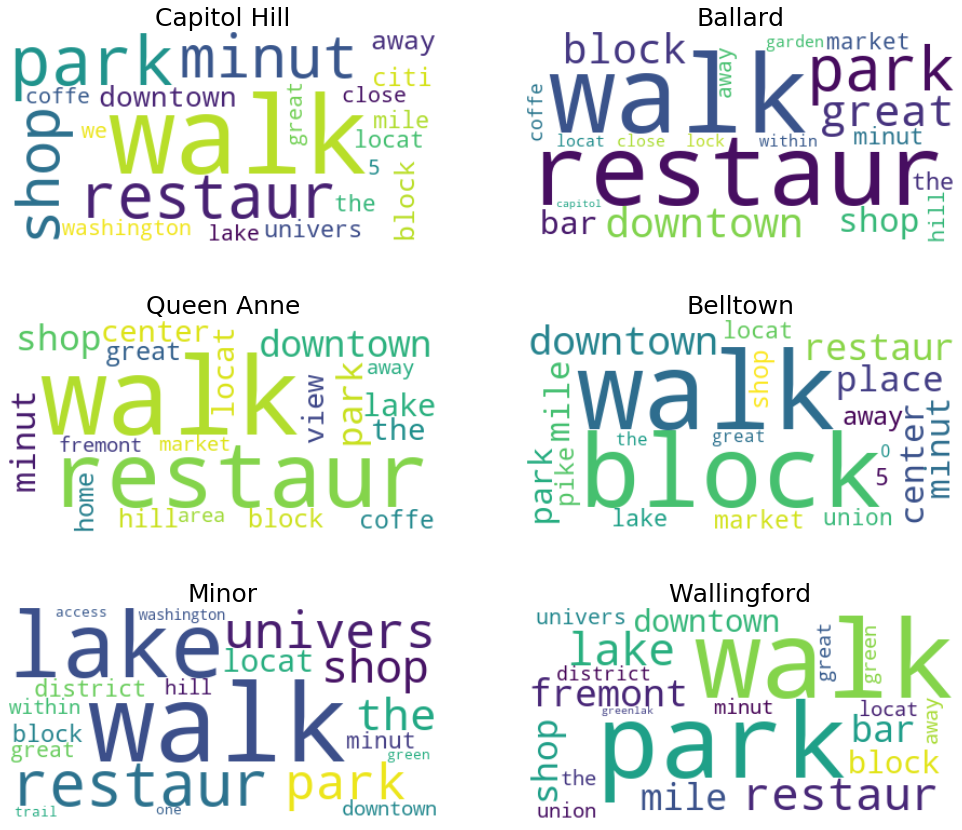
\includegraphics[width=3.5in]{photo/13_wordclouds.png}\\
  \caption{Wordclouds for the top 6 most reviewed districts}\label{wordclouds}
  \end{center}
\end{figure}
%

\subsection{Linear Regression}
\noindent Dr Liu described the Linear Regression as one of the most widely used techniques for advanced predictions. It is fundamental to more complex models, easy to interpret and easy to solve. \cite{RN7}
Linear regression attempts to model the relationship between two variables by fitting a linear equation to observed data.
The fitted line can mathematically described as:
\begin{equation}
Y_i = \beta_0 + \beta_1 X_i + \epsilon_i
\end{equation}

\begin{figure}
  \begin{center}
  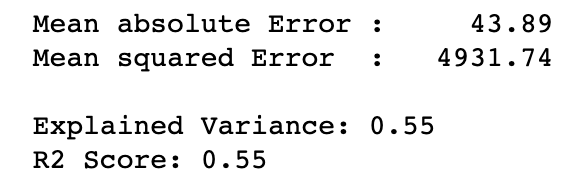
\includegraphics[width=3.5in]{photo/linear_regression.png}\\
  \caption{Errors of the Linear Regression}\label{linear_regression}
  \end{center}
\end{figure}

\subsection{Extra Tree Classifier }
\noindent The Extra Tree Classifier is a model derived from the random forest model. Decision Trees are the fundamental components of Random Forests.  Aurélien Géron says that Random Forests are among the most powerful Machine Learning algorithms available \cite{ho} . We are using it to classify the feature importance. Based on Entropy and the Information Gain, we get the essential feature\cite{Bishop} \cite{decisionforests}. Entropy and Information are defined by: 
\begin{equation}
Entropy: H(X) = -\sum p(X)\log p(X) 
\end{equation}
\begin{equation}
Information Gain: I(X,Y)= H(X)-H(X|Y)
\end{equation}
In other words, we get the feature which organizes the data the most. 

The features with the according entropy are shown in figure \ref{feature_importance}

\begin{figure}
  \begin{center}
  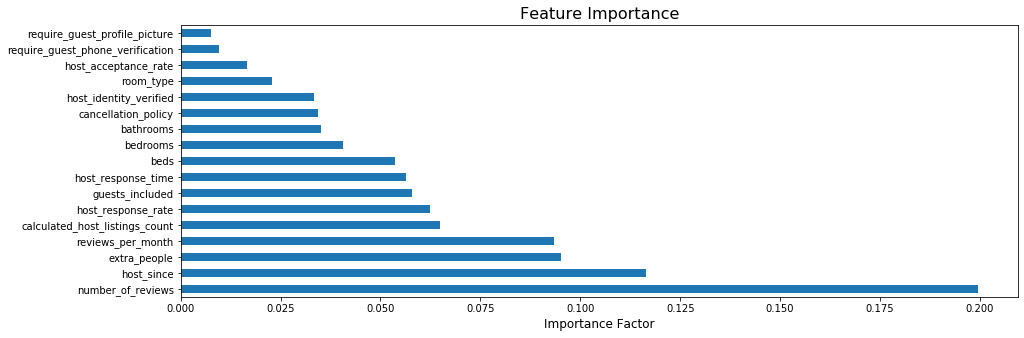
\includegraphics[width=3.5in]{photo/7_feature_importance.png}\\
  \caption{Feature Importance}\label{feature_importance}
  \end{center}
\end{figure}

This leads to the conclusion, that first leaves for predicting the price with a Tree-Classifier should be the amount of reviews. 

\begin{figure}
  \begin{center}
  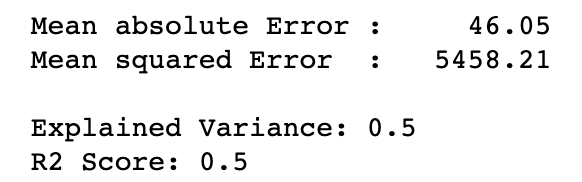
\includegraphics[width=3.5in]{photo/elastic_net.png}\\
  \caption{Errors of the Elastic Net}\label{elastic_net}
  \end{center}
\end{figure}

\subsection{Elastic Net CV}
\noindent This working paper can not explain the whole math behind the Elastic Net Classiefer, because it is to complicated. A general summary would be that the elastic net is a convex sum of ridge and lasso penalties, so the objective function for a Gaussian error model looks like:
\begin{equation}
\text{Residual MSE}+\alpha \cdot \text{Ridge Penalty}+(1-\alpha)\cdot \text{LASSO Penalty}
\end{equation}
for \(\alpha\in[0,1]\). 
So, the Elastic Net Classiefer is better as lasso and ridge regression.  It solves the limitations of both methods, while also including each as individual cases. \cite{Zou}.  
\subsection{Multinomial Naive Bayes}
\noindent The following description of the Naive Bayes is first mentioned in the book "Artificial Intelligence: A Modern Approach" from Stuart J. Russell and Peter Norvig \cite{Russell}.
The general term Naive Bayes refers the strong independence assumptions in the model, rather than the particular distribution of each feature. A Naive Bayes model assumes that each of the features it uses are conditionally independent of one another given some class. More formally, if I want to calculate the probability of observing features \(f_1\) through \(f_n\) , given some class \(c\) , under the Naive Bayes assumption the following holds:
\begin{equation}
p(f_1,..., f_n|c) = \prod_{i=1}^n p(f_i|c)
\end{equation}
This means that when I want to use a Naive Bayes model to classify a new example, the posterior probability is much simpler to work with:
\begin{equation}
p(c|f_1,...,f_n) \propto p(c)p(f_1|c)...p(f_n|c)
\end{equation}
Of course these assumptions of independence are rarely true, which may explain why some have referred to the model as the "Idiot Bayes" model, but in practice Naive Bayes models have performed surprisingly well, even on complex tasks where it is clear that the strong independence assumptions are false.\\Up to this point we have said nothing about the distribution of each feature. In other words, we have left \(p(f_i|c)\) undefined. The term Multinomial Naive Bayes simply lets us know that each \(p(f_i|c)\) is a multinomial distribution, rather than some other distribution. This works well for data which can easily be turned into counts, such as word counts in text.
\subsection{LSTM Neuronal Network}
“LSTMs,” a higher developed version of recurrent neural networks. It works, for many tasks, better than the standard version. Almost all exciting results based on recurrent neural networks are achieved with them. It’s these LSTMs that this essay will explore. Recurrent Neural Networks are too complicated for this paper \cite{olah} to explain. 

\section{Analysis}
\subsection{Why did our neural network score so much worse than the neural network of the paper \textit{Predictive modelling on Airbnb listing prices} \cite{RN1}?}
As the team of this paper \cite{RN1} mentioned in their \textit{average listing price per neighbourhood}, they figured out that the \textit{neighbourhood} has a huge impact on the price prediction. The main focus of our project was not the price prediction, but we tried to reach similar results. Our best mean absolute error is the linear regression with 43.89\$ \ref{linear_regression}. The neural network scores best for their prediction with a score of 35–32\$ \cite{RN1}. \\
We didn't have the capacity to transform the categorical neighborhood feature into a numerical one and try-out multiple neural networks. \\
Our deviation of 10\$ from their best result can be explained by that.\\
Our Network is very simple network shown in figure \ref{lstm} has a worse mean absolute error than the Linear Regression in figure \ref{nn}. 
The bad result could be explained by the missing features as already explained \cite{RN1}, but also on the not appropriate design of the network.

\begin{figure}
  \begin{center}
  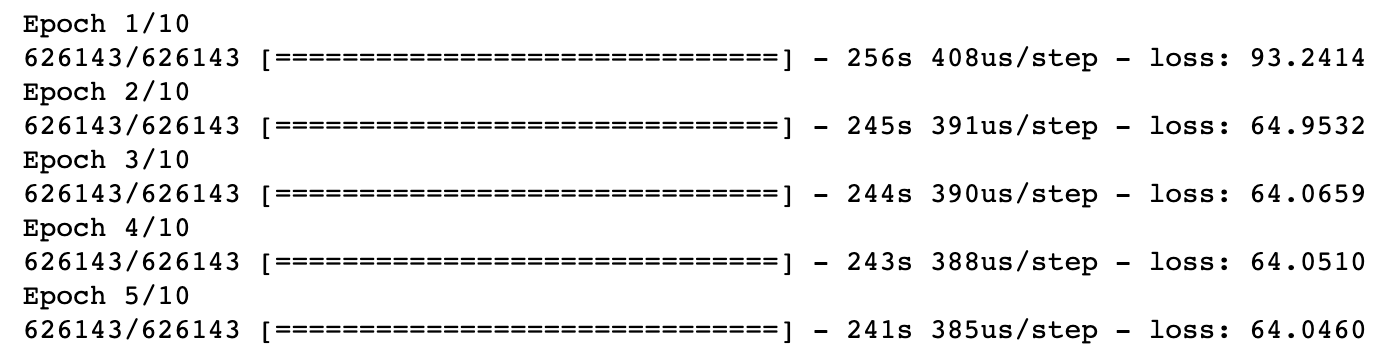
\includegraphics[width=3.5in]{photo/lstm.png}\\
  \caption{Errors of the LSTM Neural Network}\label{nn}
  \end{center}
\end{figure}
\begin{figure}
  \begin{center}
  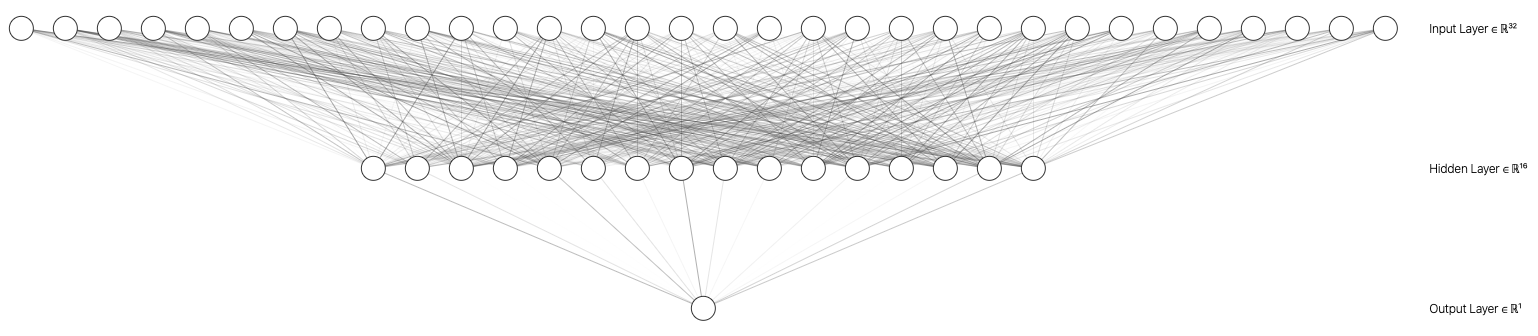
\includegraphics[width=3.5in]{photo/nn.png}\\
  \caption{LSTM Neural Network}\label{lstm}
  \end{center}
\end{figure}

\subsection{Which facts lessors need to address in their description to raise the interest of potential customer, who ‘fit’ the vibe of the neighborhood and set their focus on the same aspects as former customers of these apartments?}
In order to know what words the lessors are supposed to use in the description, we take a look at the reviews with a wordcloud. The bigger the words in the wordcloud, the more often the word was used. For example, if the customers often write the word walk in the reviews due to informing what was in walking distance of the Airbnb, the work walk will be big in the wordcloud. 
To answer this question the six most reviewed cities Capitol Hill, Ballard, Queen Anne, Belltown, Minor, Wallingford were analyzed. First, you can see that all cities have the words walk, park and restaurant written in big. The word “downtown” is also used often. For Minor, the word “lake” is very important. The rest of the words indicate that words like minute, shop, market are used often by customers. Interestingly, the word “Washington” is important for the cities Minor and Capitol Hill.


\subsection{Which price can be charged for an apartment with certain characteristics?}
First of all, we created a Linear Regression model in order to predict the price influenced by all other attributes. For this prediction we achieved a Mean Absolute Error of 44.28, which is, taking into account that the minimum rent is 10 dollar and maximum rent per night 1,650\$, very low (Figure \ref{mean_acc}). Therefore, we can assume that the listed attributes have a significant impact on the price of an accommodation and it is possible to estimate the rental price by these attributes and therefore it makes sense to use a classification tree, which takes these attributes into account.\\ In the following, we use the Extra Tree Classifier in order to find out, which attributes have a strong correlation with the price and therefore influence the price of an apartment the most. A classification tree uses the values of attributes to create groups, in which all the apartments have the same (or at least similar) values for the attributes. According to our analysis, the attributes with the highest influence on the price have a correlation coefficient in a range of 0.01 and 0.2. The highest influence on the price is the number of reviews an apartment has. This attribute has a correlation of approximately 20\%, which is almost twice as much as the second important attribute has by showing 0.112 as correlation coefficient. This attribute indicates how long the lessor is already registered as host on Airbnb. As third important factor, with a correlation coefficient of a little bit less than 0.1 the number of extra people influences the price. Other attributes which influence the price are for example the number of listings a host has/ had, number of beds, number of bath- and bedrooms. The least significant attribute in our visualization is, whether the guest needs a profile picture (with a coefficient of about 0.01). (Figure \ref{correlation-attribute-price})
\begin{figure}
  \begin{center}
  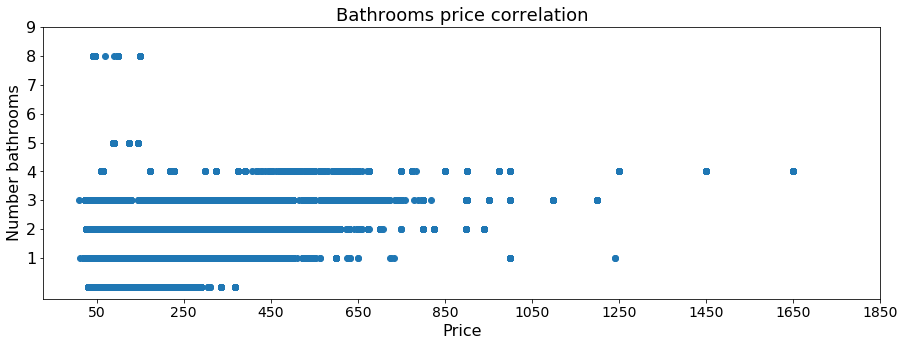
\includegraphics[width=3.5in]{photo/9_bathroom_price_correlation.png}\\
  \caption{Correlation attribute-price}\label{correlation-attribute-price}
  \end{center}
\end{figure}
In order to check that all the attributes only determine the price and do not have an influence on the price via another attribute, we also compute a heatmap to see the correlation of attributes among each other. This visualizes that host-response-time, host-response-rate and host-acceptance-rate correlate with each other and also the number of bedrooms, bathrooms and beds. So, these attributes groups influence each other and their impact on the price should be considered in a group. Furthermore, we can mention that the number of bathrooms, bedrooms and beds influence each other. So, a lessor should also take into account that if an apartment has for example a high number of bedrooms then also the number of bathrooms is high. According to this a lessor can also get some indication for the price he can charge. If his apartment has many bedrooms but only one bathroom, he can assume that other accommodations with the same number of bedrooms has more bathroom and therefore can also charge a higher price. So, this correlation is interesting for the lessors to get some price indication. (Figure \ref{heatmap })
\begin{figure}
  \begin{center}
  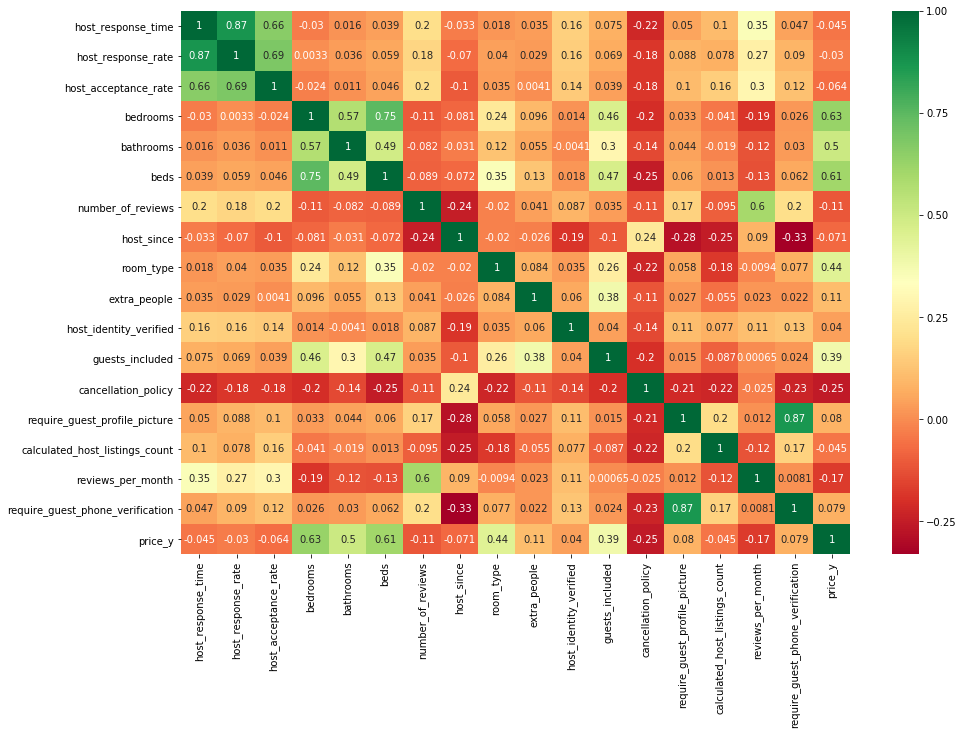
\includegraphics[width=3.5in]{photo/8_heatmap.png}\\
  \caption{Correlation attribute-price}\label{heatmap }
  \end{center}
\end{figure}
So, if a lessor wants to (re)determine the price for his accommodation, he first of all needs to consider how many reviews he got so far for the apartment. (Note: As we noted before, the reviews all give a high rating, so they are all positive. Taking this into account, it is very likely that the lessor needs to check the number of positive reviews for determining the price.) Furthermore, the lessor needs to consider how long he is already registered as host and how many people can stay in the apartment. If he considers the impact of the number of bedrooms, bathrooms and beds, he should also take into account, the correlation of the three attributes among each other.
As we already saw in figure \ref{correlation-attribute-price}, the number of beds, bedrooms and bathrooms do not have the highest impact on the price although somebody might expect, that the price is strongly influenced by these factors. \\
The same result was already shown by another paper, which further proofs those relevant features \cite{RN1}.\\ By having a closer look on the correlation between the number of bathrooms and the price as well as the number of bathroom and price, it can be recognized that an increasing number of bed- and bathrooms does not increase the entry level price within this group but only the maximal price increases. So, it is possible to find an accommodation with a different amount of bath-/ bedroom for a price of 50 dollar per night. This changes if the number of bedrooms exceeds 5. Then there is also an increase of the entry level price visible. We can conclude that the price of an apartment is probably more influenced by the fact whether it has less or more than 5 bedrooms or not. (Figure \ref{correlation-attribute-price}).

The same change can also be seen for the correlation of bathrooms and price but the change of the entry level is not that big. Therefore, the ‘strong’ change in the entry level price becomes already visible for 4 bathrooms. (Figure \ref{bathrooms-price-correlation})
\begin{figure}
  \begin{center}
  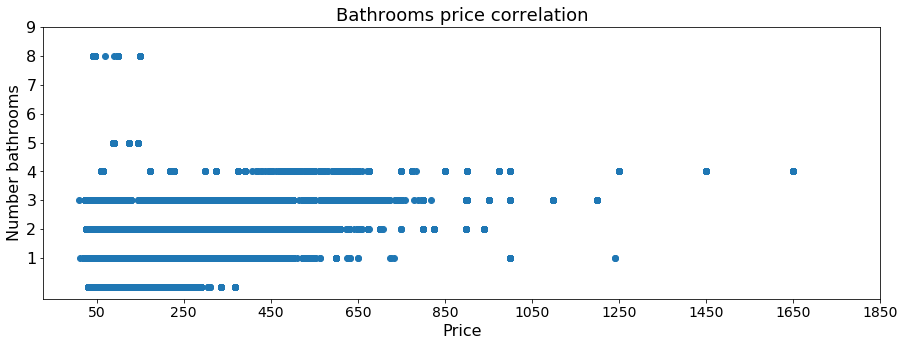
\includegraphics[width=3.5in]{photo/9_bathroom_price_correlation.png}\\
  \caption{Correlation bathrooms-price}\label{bathrooms-price-correlation}
  \end{center}
\end{figure}

\subsection{When can lessors increase the price per night for their apartment and when should they lower it?}

\begin{figure}
  \begin{center}
  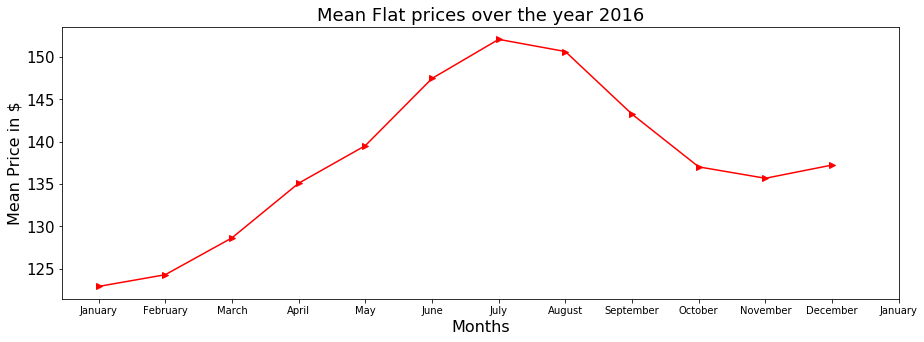
\includegraphics[width=3.5in]{photo/12_mean_flat_prices_2016.png}\\
  \caption{Mean flat prices of 2016}\label{mean_flat_prices}
  \end{center}
\end{figure}

To answer this question, we want to predict the price changes for 2017. First of all, we started by checking out the change of mean flat prices in 2016 (Figure \ref{mean_flat_prices}). 
Prices increase from January to July from about 120 to 150 dollar and decrease until November to 135 dollar. During the last month prices slightly start to increase again. It can be seen that the correlation between charged prices and the occupation ratio is rather low, as the first drop of the occupation ratio in April does not reflect in a price drop. Nevertheless, the second decrease in the number of rented apartments does reflect in the charged prices as also the price curve decreases after July. But during the month of December, prices increase as well as the number of free apartments decrease. This irregularity might be due to the fact that many people travel during Christmas time and therefore their willingness to pay is slightly increased. 

\subsection{What is a good point in time to start a marketing campaign?}

\begin{figure}
  \begin{center}
  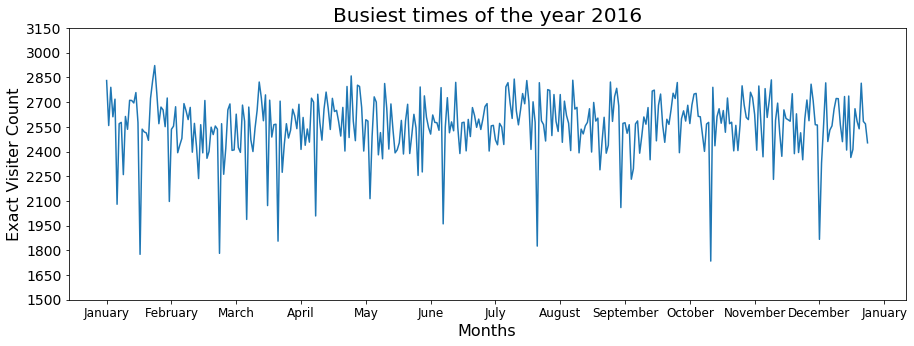
\includegraphics[width=3.5in]{photo/5_busiest_times_2016.png}\\
  \caption{Busiest times of 2016}\label{busiest_times}
  \end{center}
\end{figure}

\begin{figure}
  \begin{center}
  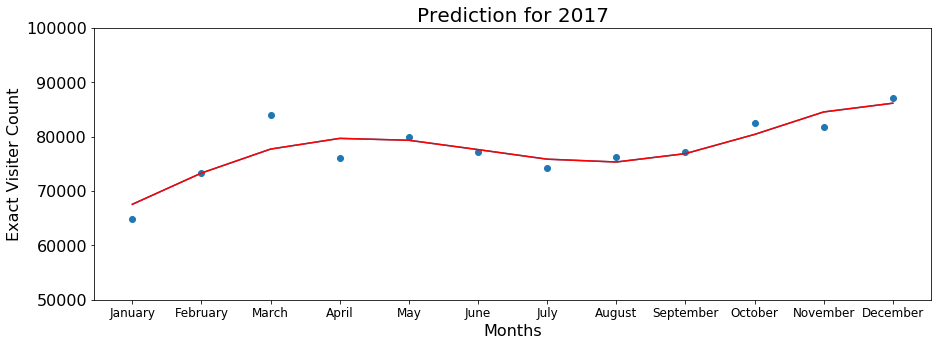
\includegraphics[width=3.5in]{photo/6_prediction_2017.png}\\
  \caption{Prediction for 2017}\label{prediction_2017}
  \end{center}
\end{figure}

\noindent In order to find the right point in time to start a marketing campaign, we need to know, during which periods the number of visitors decreases. To get some good results, we plotted a graph showing the number of visitors according to the time.\\ In Figure \ref{busiest_times} it can be seen that the number of visitors fluctuates very strong also within a month. This might be caused by changes within a week, as usually on weekends more people consider to travel and therefore more apartments are rented as well as public holidays influence the number of tourists. As exactly reflecting this fluctuation in a model would lead to a very complex model, which is expensive to create and the risk of a model overfit becomes very high, we use Linear Regression to reflect the trend of 2016 and in a second step predict the numbers of visitors for 2017. We can see that the number of visitors decreases between January and March and increases between March and July. After that there is a decrease until December. Nevertheless, the fluctuation is about 200 visitors. Compared to a total number of over 2400 visitors this change is quite small.
The predicted number of visitors can be seen in Figure \ref{prediction_2017}.\\ For 2017 it is predicted that the number of visitors raises from January to March and decreases until July. For the rest of the Year the number of visitors will raise again. So, the best point in time to start a marketing campaign would be during February till March. As the number of visitors will fall from March to July, the marketing campaign should prevent this. A campaign usually needs some time until its effectiveness can be seen so it should be started earlier than the actual decrease takes place and when the predicted decrease should take place, the effect of the campaign should keep the number of visitors on the level of March or even increase it. The campaign could be stopped in August, as its effect will last a little bit longer and between September and October the number of visitors will be on the level of March again without any campaign.

%
\section{Your findings and impacts}
\noindent We want to improve the effectiveness of marketing for Airbnb Seattle based on our findings. This can be beneficial for the lessors and Airbnb itself as Airbnb makes money off of the lessors. That means, Airbnb is only profitable if the lessors are able to rent out their listings. As a consequence, Airbnb should help the lessors to attract more visitors. \\Referring to the previous analysis one can see that the reviews are the most important factor of the consumers decision. That means the more reviews the lessors have the higher the chance their listings gets rented. This is why the lessors and Airbnb should ask their renters to write a review after they leave in order to attract more people. One should keep in mind that this report is only considering positive reviews. \\
Another suggestion for the lessors is to update their description with places that are in walking distance. Places that the renters want to visit might be shops, the metro, parks, downtown, etc. One can also mention where the renters can get food with mentioning where the nearest restaurants or cafes are. The bottom line is, the lessors should put every place into the description that is in walking distance. \\
As mentioned before, the number of reviews plays a huge part in whether a listing gets booked or not and how much can be charged. Another big factor is how long the host has been active and how many listings the host has. As those are qualities that can only be build over time, older hosts get rewarded and can charge more per listing. Consequently, lessors need to be patient in order to show that they are reliable and grow their credibility. This way their listings will get booked more often and they can charge a higher price. \\
Newer hosts can try to focus on their host\_response\_time, host\_response\_rate and host\_acceptance\_rate. As qualities like number of reviews, number of listings and how long the host has been active needs time, these are factors lessors can work on immediately in order to rent out their listing for a higher price. \\
If the host has the chance, then it is worth considering that higher number of bedrooms, bathrooms and beds can lead to people willing to pay more for the listing. That can be due to people renting the place to explore the city or work most of the time and only wanting a place to stay and shower at. This gives a reason to suspect that renters will not spend a lot of time in the Airbnb. 
We already know that the number of visitors fluctuates a lot within a month. This can be due to people visiting new places over the weekend. Consequently, it would be profitable to increase the prices from Friday to Sunday and lower them from Monday to Thursday. Moreover, it makes sense to keep the prices low from January to March before slowly increasing them from March to September. July should be the most expensive month. In December the prices can be increased again. That can be a result of holidays. Because many people decide to visit their families or go on vacation during their holidays, the demand for places to stay increases during that time period. \\
As Airbnb itself profits form their lessors renting out their places, it would be interesting to know how they can help their lessors. One way is to start campaigning at the right moment. According to the analysis, in the year 2017 the number of visitors will decrease from March to July. Meaning the marketing campaign should start in February and end in August. As Airbnb is an online platform the advertisements should be online as well. This way, possible visitors can be reached who already are comfortable using the internet. 
%
\section{Related Works}
\noindent Our main goal is the improve the effectiveness of the marketing. Nevertheless, we searched for other related papers and work and we got inspired from the question \textit{What variables in this data set are most useful in predicting the price of a particular rental?} \cite{RN2}. Not only we wanted to improve the marketing, but with the gained knowledge we also wanted to see which results we can reach with our predictions. \\
 As already mentioned, another paper reached far better results with the price prediction \cite{RN1}. \\
 A lot of further interesting plots were made on this project \cite{RN4}. Unfortunately we could not use any of this information to our advantage, but it further proofs the hypothesis of the little importance of the sentiment feature. \\
 An interesting addition for the sentiment was mentioned by Tian Lin \cite{RN3}. Regarding the (figure \ref{score_reviews_ratio}) he explained in his master thesis why people reviewed the accommodations in such a positive way. Tian explained the \textit{too-positive-phenomon} \cite{RN3}, which may be caused by the lessors themselves. Lessors apparently have the tendency to reject costumers who have the probability of reviewing in a bad way. So lessors only accept costumers with a high rate of leaving positive reviews. \\
 Further graphs and information can be found on the project \textit{How to become top earner in Airbnb?} \cite{RN5}, which is the most upvoted notebook on the Kaggle page of the Seattle dataset itself. \\
 We did not have the chance to integrate some of the results into our notebook, but this notebook shows other very interesting graphs. 
 
\section{Conclusion}
\noindent The main goal of this paper is to give some suggestions, how to apply marketing-mix strategies effectively. Hereby the focus is on the Product, Price and Promotion policy.\\
Regarding the Product policy the paper shows, it is of interest which characteristics of the accommodations visitors’ value high. In order to obtain a clearer result, the six neighborhoods with the highest number of reviews, were analyzed. A result should be obtained by conducting a word cloud which displays the most used 50 word within all reviews. The size of the displayed words depended on the number of occurrences of this word in a review for the particular neighborhood. The analysis shows that especially words like "walk", "park", "lake", "downtown", "minute", "shop" and "market" occur quite often. Lessors should definitely include these words in their description in order to make sure to address the right people, who will enjoy their stay in the apartment and the surrounding area. This has the positive impact that a satisfied customer will use Airbnb also for his next booking of accommodation, which increases the revenue of Airbnb. As the analysis shows, most of the reviews are very positive. So it might also exist a correlation between the satisfaction of a customer and whether he writes a review or not. If this is the case, it can be assumed that a satisfied customer will write a positive review and this will be positive for the lessor, as his number of reviews increases, which increases the price the lessor can charge. This is automatically a question, which can be kept in mind for further investigation. To check whether there really exists a correlation between these two variables or not and if there is a connection, why it exists.\\
By using a Linear Regression and a Extra Tree Classifier, the correlation between different attributes and price has been analyzed. The result showed that first of all there is a correlation and secondly the price depends the strongest of the number of reviews. This is the reason why, it has been concluded before that if the right customer group has been addressed and satisfied customers write a review the price the lessor can charge can increase. Increased prices will also cause an increase in the revenue of Airbnb, which has to be considered as positively for shareholders. Other factors, which influence the price are: number of bedrooms, number of beds, number of bathrooms and length of registered as host. Here it has to be mentioned that number of bedrooms, beds and bathrooms also correlate with each other. So, if analyzing and evaluating the price for a new apartment, this has to be kept in mind. Furthermore, it can be mentioned that the number of bedrooms needs to exceed 5 before the entry price is increased. For the number of bathrooms 4 are sufficient to change the entry price. In a next step, if further has been analyzed by a Linear Regression, when prices can be increased. During January till July prices lessors can increase but need to decrease the prices until November. In month of December prices increase again.\\
To answer the question when a marketing campaign should be started the degree of booking is taken in consideration. The number of customers increases from January to Murch but then the number drops. So, it makes since to start a campaign in February so its effect will be noticeable in March and then prevents the number of visitors from decreasing. The campaign can be stopped in August, when the number of visitors starts to raise again to the level of bevor.\\
Another aspect which can be dealt with in future analysis is, whether the attributes of the dataset can also be used to draw a conclusion on the correlation between several attributes and the degree of booking. This is also interesting, as the results can be compared with this analysis and it can be compared, whether the influencing attributes are similar.





\section*{Acknowledgment}
\noindent The authors would like to thank Dr. Liu Junming from the City University of Hongkong for a really good supervising of our group. Dr. Liu helped us so much and we wouldn't have reached this result without him. 



% if have a single appendix:
%\appendix[Proof of the Zonklar Equations]
% or
%\appendix  % for no appendix heading
% do not use \section anymore after \appendix, only \section*
% is possibly needed

% use appendices with more than one appendix
% then use \section to start each appendix
% you must declare a \section before using any
% \subsection or using \label (\appendices by itself
% starts a section numbered zero.)
%

% ============================================
%\appendices
%\section{Proof of the First Zonklar Equation}
%Appendix one text goes here %\cite{Roberg2010}.

% you can choose not to have a title for an appendix
% if you want by leaving the argument blank
%\section{}
%Appendix two text goes here.


% use section* for acknowledgement
%\section*{Acknowledgment}


%The authors would like to thank D. Root for the loan of the SWAP. The SWAP that can ONLY be usefull in Boulder...


% Can use something like this to put references on a page
% by themselves when using endfloat and the captionsoff option.
\ifCLASSOPTIONcaptionsoff
  \newpage
\fi



% trigger a \newpage just before the given reference
% number - used to balance the columns on the last page
% adjust value as needed - may need to be readjusted if
% the document is modified later
%\IEEEtriggeratref{8}
% The "triggered" command can be changed if desired:
%\IEEEtriggercmd{\enlargethispage{-5in}}

% ====== REFERENCE SECTION

%\begin{thebibliography}{1}

% IEEEabrv,

\bibliographystyle{IEEEtran}
\bibliography{IEEEabrv,Bibliography}
%\end{thebibliography}
% biography section
% 
% If you have an EPS/PDF photo (graphicx package needed) extra braces are
% needed around the contents of the optional argument to biography to prevent
% the LaTeX parser from getting confused when it sees the complicated
% \includegraphics command within an optional argument. (You could create
% your own custom macro containing the \includegraphics command to make things
% simpler here.)
%\begin{biography}[{\includegraphics[width=1in,height=1.25in,clip,keepaspectratio]{mshell}}]{Michael Shell}
% or if you just want to reserve a space for a photo:

% ==== SWITCH OFF the BIO for submission
% ==== SWITCH OFF the BIO for submission


%% if you will not have a photo at all:
%\begin{IEEEbiographynophoto}{Ignacio Ramos}
%(S'12) received the B.S. degree in electrical engineering from the University of Illinois at Chicago in 2009, and is currently working toward the Ph.D. degree at the University of Colorado at Boulder. From 2009 to 2011, he was with the Power and Electronic Systems Department at Raytheon IDS, Sudbury, MA. His research interests include high-efficiency microwave power amplifiers, microwave DC/DC converters, radar systems, and wireless power transmission.
%\end{IEEEbiographynophoto}

%% insert where needed to balance the two columns on the last page with
%% biographies
%%\newpage

%\begin{IEEEbiographynophoto}{Jane Doe}
%Biography text here.
%\end{IEEEbiographynophoto}
% ==== SWITCH OFF the BIO for submission
% ==== SWITCH OFF the BIO for submission



% You can push biographies down or up by placing
% a \vfill before or after them. The appropriate
% use of \vfill depends on what kind of text is
% on the last page and whether or not the columns
% are being equalized.

\vfill

% Can be used to pull up biographies so that the bottom of the last one
% is flush with the other column.
%\enlargethispage{-5in}



% that's all folks
\end{document}